% Preamble
% ---
\documentclass[12pt]{article}

% Misc Packages
% ---
\usepackage[utf8]{inputenc}
\usepackage[english]{babel}

% Page Margins (and size)
% ---
\usepackage{geometry}
\geometry{letterpaper, portrait, margin=1in}

% Paragraph spacing
\setlength{\parskip}{1em}

% Double space the lines
\linespread{2}

% PNG image import
\usepackage{graphicx}

% Main Document
% ---
\begin{document}

\noindent Derek Gonyeo \hfill \today \\
Final Paper \hfill Humans and their Environments

\begin{center}
    \huge Reproducibility in Archaeological Discoveries
\end{center}

\normalsize

% Intro
% - archaeological discoveries aren't reproducible
% - random example
%
% A way forward
% - Marwick's paper
% - 4 steps
%
% His case study
% - 1989 expedition recovered some stuff
% - stone artefacts never described in detail, leading to doubts
% - part of a study (2015) to study this stuff
% - went over tools he used for reproducibility
%
% Issues with adoption
% - 3 points
%
% OpenABM
% - Specified processes for ABM research
% - Paper before
% - Paper after
%
% Next Steps
% - Find a paper with open data
% - Reproduce the results
% - Write about it

Peer review is a critical process for any scientific discovery. When a
researcher produces a paper containing their work, the paper is then
scrutinized by other professionals in the same field before it is published.
This process exists to help verify that the new discoveries are the production
of rigorous and methodical work, and that the facts and conclusions presented
by the paper are sound. 

In hard sciences, like mathematics or chemistry, it is usually clear what steps
are necessary to follow to verify a given discovery. For mathematics, derive a
proof for whatever new relation was discovered. In chemistry, reproduce
whatever new reaction was found.

In archaeology, the steps necessary to reproduce a given discovery are nowhere
near as obvious. When an archaeologist discovers some new facet of an ancient
civilization through an excavation, ideally one of their peers could return to
the site and perform the same excavation. Alas the very nature of an excavation
is to irreparably destroy the site, not to mention the time, money, manpower,
and organization required to perform an excavation.

Despite the impossibility of perfectly reproducing an excavation, the analysis
that takes place on the artefacts and measurements obtained during the
excavation has no such restriction. So long as the data recovered from
excavations is assumed to have been produced truthfully and with rigorous
techniques, archaeological discoveries should thus be reproducible through
inspections and reconstructions of the analysis performed.

Unfortunately the majority of published archaeological papers don't make their
datasets available, and those that do often fail to sufficiently document the
decisions made in the transformations and analysis of the data.

In January of 2016 Ben Marwick published a paper titled "Computational
Reproducibility in Archaeological Research: Basic Principles and a Case Study
of their Implementation" \cite{marwick16}. In this paper he borrows some tools
from the field of software engineering in an attempt to address this issue, and
ultimately outlines four principles that could be applied to archaeological
research to improve reproducibility. This paper will outline and detail these
principles, identify their impact on a case study on their implementation done
by Marwick, and attempt to identify and address issues with their widespread
adoption in the field.

These principles are as follows: to publish the datasets collected for the
research, perform analysis on these datasets with computer scripts, use version
control to help manage the files in the project, and to provide a consistent
computational environment to guarantee that the scripts will be usable in the
future.

The first of these principles, to publish the datasets developed during the
research, requires little planning or additional background knowledge, and
consideration of this may even be deferrable until after publication of the
research. This principle will also result in the largest rewards of any of the
principles, as Marwick enumerates many studies which have shown that papers
that make their datasets available enjoy higher numbers of citations.

The second of these principles, to perform analysis via computer scripts, stems
from a handful of reasons. Scientific research in general has been trending
towards using computation to perform analysis, and archaeology is no exception.
Unfortunately graphical user applications like Excel do not lend themselves
well to reproducibility, as recording a series of operations (e.g. button
clicks) isn't particularly easy and the user interfaces will change over time.
A script on the other hand records the steps it performs by its very nature; a
script is a list of steps for the computer to perform to carry out the
analysis. There are also quantifiable benefits to individual researchers for
doing computation through scripts, as they benefit from freely available code
produced by other researchers.

The third principle doesn't directly improve research reproducibility, and
instead exists as advice to simplify project management. Version control
software is a tool commonly employed by software engineers, and allows changes
to files to be tracked and accounted for. Using such a tool allows access to
the state of the project at any point in time. If the scripts are discovered to
have broken due to some change, it is easy to simply restore a previous version
of the script before the harmful change was introduced.

The fourth principle, to provide a consistent computational environment, lacks
quantifiable benefits to the researcher but will assist their peers in
reproducing their work. This has traditionally been done with virtual machines,
but lately a more practical tool referred to as Linux containers has been
gaining popularity among software engineers.

These principles were applied during a paper that Marwick assisted in
producing. Focusing on a site in northern Australia called Madjedbebe, the
authors performed an analysis on stone and faunal artefacts obtained during an
excavation in 1989. The objective was to verify the stratigraphic integrity of
the original excavation and corresponding analysis, which demonstrated that the
site had human occupation between 50 and 60 thousand years ago
\cite{clarkson15}.

This paper does briefly mention that the analysis and visualization of the data
was performed with R scripts, and provides a URL to where the data and source
code can be accessed. Aside from the short mention of these methods before
launching into a presentation of the results, the paper doesn't otherwise
discuss or mention the computational approach to analysis.

In Marwick's paper on reproducibility, he describes what tools he used in the
Madjedbebe study to accomplish each of his four principles. To publish the
dataset he used Figshare, which provides file hosting services tailored
specifically for academic research. Figshare is not specific to archaeological
research, and there are online services that are, but Figshare provides free
unlimited archiving of any file type, so long as each file is less than 250 MB
in size.

To achieve his second principle of performing analysis with scripts, Marwick
used the programming language R. This language is popular among researchers in
various other disciplines, and is heavily geared towards data analysis and
visualization. Notably the language is used extensively among statisticians,
which has the nice result of a wide selection of statistical algorithms freely
available in the language.

As for version control and a consistent computational environment, git and
docker were respectively chosen. Both have the benefit of being widely used by
software engineers, and thus have extensive documentation and there exist
services that will freely host git repositories and docker images.

Marwick also discusses the practicality of a typical archaeologist using these
technologies. To do so, an archaeologist must become proficient in both
programming and related tools. Marwick states that he spent 3 years teaching
himself how to use R, which is probably a time commitment most archaeologists
would balk at (that's over half the time it takes to get an undergraduate
degree). Even were an archaeologist to invest the time to learn these tools,
one issue Marwick faced was a very uneven distribution of work among the
researchers in the Madjedbebe study. Those more familiar with R were much more
heavily involved in the final analysis than those who were less capable with
the tool.

Fortunately, 3 years is likely a much longer time than is necessary to develop
a familiarity with R. Marwick himself suspects that that competence could be
developed "substantially quicker" than 3 years by taking short training
courses. There are already multiple organizations offering such courses, like
Software Carpentry and rOpenSci. Marwick also holds the opinion that once the
technologies are learned, applying them will take no longer than alternative
techniques and may even offer some time savings due to the fact that code
produced by past efforts is often reusable.

Even if training archaeologists to program was trivial, realistically any
processes to address reproducibility won't be adopted without a mandate,
presumably from the journals. Luckily the discipline has already demonstrated
it can quickly adopt new processes when necessary, as happened roughly a decade
ago.

In 2006 Grimm et al. published "A standard protocol for describing
individual-based and agent-based models", which outlines a standard protocol
for the presentation of research based on agent-based modeling. This was the
ODD protocol, which is an acronym for Overview, Design concepts, and Details
\cite{grimm06}.  Since the publication, this protocol has been widely adopted
by many disciplines, archaeology included. Organizations like OpenABM have even
appeared to support this process.

Were other processes to be standardized and imposed on archaeologists, in the
name of reproducibility, the adoption of the ODD protocol shows that they can
be accepted by the discipline.

As a specific requirement for journals to impose on researchers, Marwick
suggests that a research compendia be required alongside any paper presented
for publication. Such a compendia would include at a minimum the manuscript and
dataset produced during the research, and potentially also files such as the
suggested scripts to perform analysis on the data.

To explore a practical application of these concepts, I sought to find an
archaological paper that has a published dataset, and aside from this has not
adhered to any of the other principles outlined by Marwick. With the paper and
dataset, I would create a script that would ingest the published dataset and
programmatically reproduce a subset of the analysis performed by the paper.

After a brief search, I found a paper titled "Food for Rome: A Stable Isotope
Investigation of Diet in the Imperial Period (1st-3rd Centuries AD)" that
utilizes a dataset published on figshare.com \cite{killgrove13}.

This paper performed a stable isotope analysis on skeletons found in cemeteries
around Rome, Italy dating back to the 1st to 3rd centuries AD. The analysis
aimed to establish if there were differing diets between non-upper-class
members of ancient Roman society based on varying factors like gender and urban
vs suburban environments.

The cemeteries sourced for skeletons were Casal Bertone, which was very close
to the city of Rome, and Castellaccio Europarco, which was close to the edge of
the 50 km radius that defined the suburbium around the city. In Castellaccio
Europarco, the skeletons were also divided between a necropolis and a
mausoleum, with the mausoleum samples likely belonging to what were wealthier
individuals in ancient Roman society.

Based on the analysis performed by the authors, they found that individuals
from an urban environment (the skeletons from Casal Bertone) favored aquatic
foods, while individuals from a more suburban environment ate much more
millet-based foods. There were no discernible differences in diet between the
genders.

I decided to attempt to reproduce figure 2 in the paper, which graphed the
carbon isotopes versus the nitrogen isotopes on a scatter plot for skeletons
from both locations. My objective was to use a script written in Python to read
in data from the excavation and produce an image of the graph in the figure.

In order to attempt to reproduce this graph, I of course needed the data, which
I downloaded from figshare. I however immediately encountered an issue with my
plan, as the data was stored in a .mdb file, which is the format used by
Microsoft Access. As I don't have Microsoft Office, it took quite some time to
figure out how to access this data. Python has tools to read data out of a
Microsoft Access file, but these tools only work when run on a Windows
computer, whereas my laptop is running Linux. After much searching for a tool,
I managed to write a Python script that, when combined with an external tool on
Linux, was able to export the data into CSV files.

This little adventure in being able to get the data into a format I could work
with was very interesting, as Marwick does mention that when data is published
it is ideally made available in an easy to use format, and calls out CSV
specifically as a good format. The idea behind his suggestion is that if your
data can't be viewed by the reader, its usefulness is greatly reduced.
Microsoft Access files are not portable at all, and will only be readable on
Windows machines, whereas the CSV format is supported on a myriad of systems
(Microsoft Excel included) \cite{marwick16}.

With the data in CSV, I wrote a Python script that reads in one of the tables,
filters out all rows that don't include values for every necessary field for
the graph, and then saves out a PNG file with the graphed data. This is the
resulting graph:

\begin{center}
    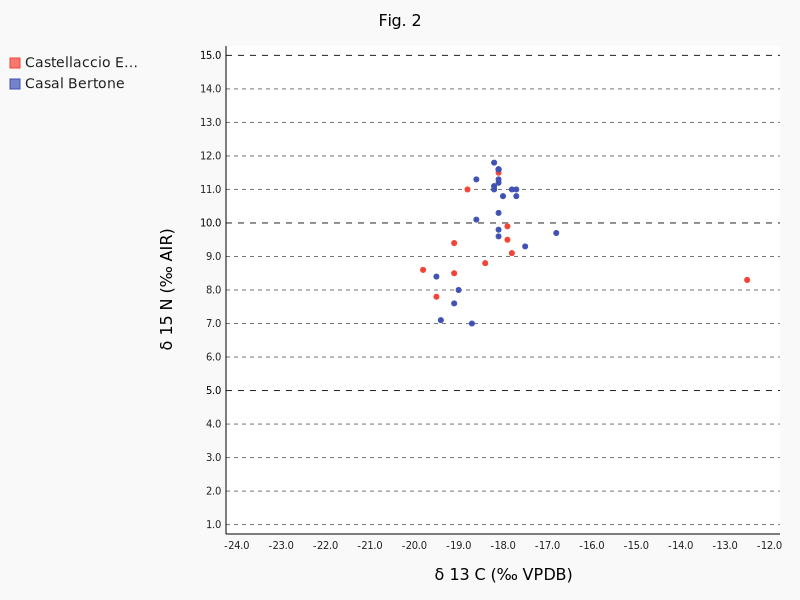
\includegraphics[width=5in, keepaspectratio]{fig2} \\
    A programmatically generated version of figure 2 from "Food for Rome"
    \cite{killgrove13}.
\end{center}

Missing from the graph is all of the data points from the animals, and there's
no distinction between samples from the mausoleum and the necropolis in Casal
Bertone. The table in the published dataset that I used to produce the graph
included no data on animals, and the table made no distinction between the two
locations for skeletons from Casal Bertone.

Aside from the missing datapoints, the graph does exactly represent figure 2
from "Food for Rome". By inspection of the code that generates the graph, which
should be a fairly trivial process for someone familiar with Python as the
script in its entirety is 25 lines, it's clear how the graph is produced from
the dataset.

I would also liked to have reproduced figure 4 from the paper, as it features
distinct groupings of points that are visually recognizable, and clearly
demonstrates a notable difference between the groups, I decided not too as I
did not know the values for the protein lines plotted on the graph.

For all of the situations in which I did not know the source of some of the
data in the graphs presented by the paper, the animal data in figure 2, the
distinction between the skeleton locations from Casal Bertone in figure 2, and
the values for the protein lines in figure 4, my answers would have been easily
discoverable had the graphs been produced by auditable scripts. In the current
state of affairs, I do not know how the graphs are generated and where or how
the data I am lacking in my graph comes from.

The python script used for this paper, in addition to the source for my paper
itself, is available at
\texttt{https://github.com/dgonyeo/humans-and-their-environment}.

This application of Marwick's principles hopefully illustrates the benefits of
programmatically performing one's analysis, as multiple aspects of the graphs
"Food for Rome" presents would have been much clearer to me had there been a
script that would generate the graphs.

\newpage
\begin{thebibliography}{9}
    \bibitem{marwick16}
        Marwick, Ben.
        "Computational Reproducibility in Archaeological Research: Basic Principles and a Case Study of Their Implementation."
        \textit{Journal of Archaeological Method and Theory}
        (2016): n. pag. Web.

    \bibitem{clarkson15}
        Clarkson, Chris,
        Mike Smith,
        Ben Marwick,
        Richard Fullagar,
        Lynley A. Wallis,
        Patrick Faulkner,
        Tiina Manne,
        Elspeth Hayes,
        Richard G. Roberts,
        Zenobia Jacobs,
        Xavier Carah,
        Kelsey M. Lowe,
        Jacqueline Matthews,
        and S. Anna Florin.
        "The Archaeology, Chronology and Stratigraphy of Madjedbebe (Malakunanja II): A Site in Northern Australia with Early Occupation."
        \textit{Journal of Human Evolution}
        83 (2015): 46-64. Web.

    \bibitem{grimm06}
        Grimm, Volker,
        Uta Berger,
        Finn Bastiansen,
        Sigrunn Eliassen,
        Vincent Ginot,
        Jarl Giske,
        John Goss-Custard,
        Tamara Grand,
        Simone K. Heinz,
        Geir Huse,
        Andreas Huth,
        Jane U. Jepsen,
        Christian Jørgensen,
        Wolf M. Mooij,
        Birgit Müller,
        Guy Pe’Er,
        Cyril Piou,
        Steven F. Railsback,
        Andrew M. Robbins,
        Martha M. Robbins,
        Eva Rossmanith,
        Nadja Rüger,
        Espen Strand,
        Sami Souissi,
        Richard A. Stillman,
        Rune Vabø,
        Ute Visser,
        and Donald L. Deangelis.
        "A Standard Protocol for Describing Individual-based and Agent-based Models."
        \textit{Ecological Modelling}
        198.1-2 (2006): 115-26. Web.

    \bibitem{killgrove13}
        Killgrove, Kristina,
        and Robert H. Tykot.
        "Food for Rome: A Stable Isotope Investigation of Diet in the Imperial Period (1st–3rd Centuries AD)."
        \textit{Journal of Anthropological Archaeology}
        32.1 (2013): 28-38. Web.

\end{thebibliography}

\end{document}
